\section{Sprint 1}
Tal y como se ha definido en la sección \ref{sec:planificacion-inicial}, el primer sprint se centra en la base de nuestra aplicación web, desarrollando la estructura inicial del servidor, gestión de usuarios y subida y descarga sencilla de archivos.
Para ello, se han elegido las historias de usuario relacionadas con el objetivo de este sprint y se han desarrollado definiendo sub-historias de usuario si fueran necesarias, criterios de aceptación y las tareas necesarias para su implementación.

Las historias de usuario se han seleccionado de manera aproximada, puesto que al ser el primer sprint no tenemos una velocidad de equipo definida. Existe la posibilidad de que algunas historias de usuario no se completen en este sprint o de que se completen más de las previstas, por lo que se ha dejado un margen de maniobra para que el equipo pueda adaptarse a la realidad del desarrollo.

Cuando se termine el sprint, se calculará la velocidad del equipo la cual se utilizará para planificar los siguientes sprints, de manera que se pueda ajustar la cantidad de historias de usuario a desarrollar en cada uno de ellos.

Una vez definidas todas las tareas que se van a realizar en este sprint, se ha realizado un diagrama de Gantt para planificar el tiempo que se va a dedicar a cada una de ellas, teniendo en cuenta que el sprint tiene una duración de dos semanas, y se dará un orden de prioridad a las tareas que se consideren más importantes para llegar a el objetivo del sprint.

\subsection{Historias de usuario}
En esta sección se detallan las historias de usuario y técnicas que se han elegido para este sprint. Se va a hacer una breve descripción de cada una de ellas, así como los criterios de aceptación y las tareas necesarias para su implementación. Si fuera necesario, se definirán sub-historias de usuario para facilitar su desarrollo.

Las seleccionadas son las siguientes:
\begin{itemize}
    \item HU05: Inicio de sesión - 5 PH
    \item HU06: Cerrar sesión - 2 PH
    \item HU13: Crear cuentas - 8 PH
    \item HT03 API REST en Rust - 13 PH
    \item HT05: Autenticación JWT - 5 PH
    \item HT08: Base de datos - 8 PH
    \item HT18.1: Binario - 2 PH
    \item HT19: Dockerización - 3 PH
    \item HT20.1: Documentación del proyecto en GitHub - 5 PH
    \item HT20.2: Documentación de la API REST con OpenAPI - 5 PH
\end{itemize}

Estas historias de usuario y técnicas suman un total de 56 puntos de historia (PH). Es importante destacar que la estimación en puntos de historia representa la complejidad relativa de cada historia, mientras que las tareas de desarrollo se estiman en horas de trabajo efectivo.

\paragraph{Descomposición en tareas de desarrollo}

% HU05: Inicio de sesión
\begin{table}[H]
    \begin{center}
        \begin{tabularx}{\textwidth}{|l|X|l|}
            \hline
            \textbf{Identificador HU05} & 
            \textbf{Como usuario, quiero iniciar sesión con contraseña o clave, para evitar que otros accedan a mis archivos} &
            \textbf{Estimación: 5 PH}\\
            \hline
            \multicolumn{3}{|p{\textwidth}|}{
                \begin{minipage}{\textwidth}
                    \centering
                    \vspace{0.5em}
                    \begin{tabular}{|l|p{8cm}|r|}
                        \hline
                        \textbf{Identificador} & \textbf{Título de la tarea de desarrollo} & \makecell{\textbf{Estimación}\\\textbf{(h)}} \\
                        \hline
                        Tarea 5-1 & Implementar endpoint para iniciar sesión & 2 \\
                        \hline
                        Tarea 5-2 & Validar credenciales de usuario contra la base de datos & 1.5 \\
                        \hline
                        Tarea 5-3 & Generar y devolver token JWT al usuario autenticado & 1.5 \\
                        \hline
                        Tarea 5-4 & Gestionar errores de autenticación (usuario no existe, contraseña incorrecta) & 1.5 \\
                        \hline
                        Tarea 5-5 & Documentar el endpoint de inicio de sesión en OpenAPI & 0.5 \\
                        \hline
                    \end{tabular}
                    \vspace{0.5em}
                \end{minipage}
            } \\
            \hline
            \multicolumn{3}{|p{\textwidth}|}{
                \textbf{Pruebas de aceptación:}
                    \begin{itemize}
                        \item El usuario puede iniciar sesión con su contraseña.
                        \item Cuando el usuario inicia sesión, se le devuelve un token JWT.
                        \item Si el usuario no existe, se devuelve un mensaje de error.
                        \item Si la contraseña o clave son incorrectas, se devuelve un mensaje de error.
                        \item El endpoint está documentado en OpenAPI.
                    \end{itemize}
            }\\
            \hline
            \multicolumn{3}{|p{\textwidth}|}{
                \textbf{Observaciones:}
                \begin{itemize}
                    \item El endpoint debe ser seguro (usar HTTPS).
                    \item El token JWT debe tener expiración configurable.
                \end{itemize}
            }\\
            \hline
        \end{tabularx}
    \end{center}
\end{table}

% HU06: Cerrar sesión
\begin{table}[H]
    \begin{center}
        \begin{tabularx}{\textwidth}{|l|X|l|}
            \hline
            \textbf{Identificador HU06} & 
            \textbf{Como usuario, quiero poder cerrar sesión en un dispositivo, para proteger mis datos si pierdo el móvil} &
            \textbf{Estimación: 2 PH}\\
            \hline
            \multicolumn{3}{|c|}{
                \begin{minipage}{\linewidth}
                    \centering
                    \vspace{0.5em}
                    \begin{tabular}{|l|p{8cm}|r|}
                        \hline
                        \textbf{Identificador} & \textbf{Título de la tarea de desarrollo} & \makecell{\textbf{Estimación}\\\textbf{(h)}} \\
                        \hline
                        Tarea 6-1 & Implementar endpoint para cerrar sesión (invalidar token JWT) & 1 \\
                        \hline
                        Tarea 6-2 & Gestionar lista negra de tokens JWT (opcional) & 1 \\
                        \hline
                    \end{tabular}
                    \vspace{0.5em}
                \end{minipage}
            } \\
            \hline
            \multicolumn{3}{|p{\textwidth}|}{
                \textbf{Pruebas de aceptación:}
                    \begin{itemize}
                        \item El usuario puede cerrar sesión y su token queda invalidado.
                        \item Tras cerrar sesión, el token no permite acceder a endpoints protegidos.
                    \end{itemize}
            }\\
            \hline
            \multicolumn{3}{|p{\textwidth}|}{
                \textbf{Observaciones:}
                \begin{itemize}
                    \item Si no se implementa lista negra, el token expira por tiempo.
                \end{itemize}
            }\\
            \hline
        \end{tabularx}
    \end{center}
\end{table}

% HU13: Crear cuentas
\begin{table}[H]
    \begin{center}
        \begin{tabularx}{\textwidth}{|l|X|l|}
            \hline
            \textbf{Identificador HU13} & 
            \textbf{Como administrador, quiero crear cuentas de usuario con permisos, para que varias personas puedan usar el servidor} &
            \textbf{Estimación: 8 PH}\\
            \hline
            \multicolumn{3}{|c|}{
                \begin{minipage}{\linewidth}
                    \centering
                    \vspace{0.5em}
                    \begin{tabular}{|l|p{8cm}|r|}
                        \hline
                        \textbf{Identificador} & \textbf{Título de la tarea de desarrollo} & \makecell{\textbf{Estimación}\\\textbf{(h)}} \\
                        \hline
                        Tarea 13-1 & Implementar endpoint para crear cuentas de usuario & 2 \\
                        \hline
                        Tarea 13-2 & Validar permisos de administrador para crear cuentas & 1.5 \\
                        \hline
                        Tarea 13-3 & Añadir roles/permisos a los usuarios & 1.5 \\
                        \hline
                        Tarea 13-4 & Gestionar almacenamiento seguro de contraseñas (hash) & 1.5 \\
                        \hline
                        Tarea 13-5 & Documentar el endpoint de creación de cuentas en OpenAPI & 0.5 \\
                        \hline
                        Tarea 13-6 & Pruebas unitarias de creación de usuario & 1 \\
                        \hline
                    \end{tabular}
                    \vspace{0.5em}
                \end{minipage}
            } \\
            \hline
            \multicolumn{3}{|p{\textwidth}|}{
                \textbf{Pruebas de aceptación:}
                    \begin{itemize}
                        \item Solo el administrador puede crear cuentas.
                        \item El usuario creado puede iniciar sesión.
                        \item Los roles/permisos se asignan correctamente.
                        \item El endpoint está documentado en OpenAPI.
                    \end{itemize}
            }\\
            \hline
            \multicolumn{3}{|p{\textwidth}|}{
                \textbf{Observaciones:}
                \begin{itemize}
                    \item Usar hash seguro para contraseñas (ej: Argon2).
                \end{itemize}
            }\\
            \hline
        \end{tabularx}
    \end{center}
\end{table}

% HT03: API REST en Rust
\begin{table}[H]
    \begin{center}
        \begin{tabularx}{\textwidth}{|l|X|l|}
            \hline
            \textbf{Identificador HT03} & 
            \textbf{Desarrollar API RESTful usando Rust y Axum} &
            \textbf{Estimación: 13 PH}\\
            \hline
            \multicolumn{3}{|c|}{
                \begin{minipage}{\linewidth}
                    \centering
                    \vspace{0.5em}
                    \begin{tabular}{|l|p{8cm}|r|}
                        \hline
                        \textbf{Identificador} & \textbf{Título de la tarea de desarrollo} & \makecell{\textbf{Estimación}\\\textbf{(h)}} \\
                        \hline
                        Tarea 3-1 & Crear estructura base del proyecto en Rust & 2 \\
                        \hline
                        Tarea 3-2 & Configurar Axum y dependencias principales & 2 \\
                        \hline
                        Tarea 3-3 & Definir rutas y controladores básicos & 2 \\
                        \hline
                        Tarea 3-4 & Implementar manejo de errores global & 2 \\
                        \hline
                        Tarea 3-5 & Añadir middlewares (logging, CORS, etc.) & 1.5 \\
                        \hline
                        Tarea 3-6 & Configurar variables de entorno y settings & 1.5 \\
                        \hline
                        Tarea 3-7 & Documentar endpoints iniciales & 1 \\
                        \hline
                        Tarea 3-8 & Pruebas de integración básicas & 1 \\
                        \hline
                    \end{tabular}
                    \vspace{0.5em}
                \end{minipage}
            } \\
            \hline
            \multicolumn{3}{|p{\textwidth}|}{
                \textbf{Pruebas de aceptación:}
                    \begin{itemize}
                        \item El servidor arranca y responde a peticiones básicas.
                        \item Los endpoints definidos funcionan correctamente.
                        \item El manejo de errores es consistente.
                    \end{itemize}
            }\\
            \hline
            \multicolumn{3}{|p{\textwidth}|}{
                \textbf{Observaciones:}
                \begin{itemize}
                    \item Seguir estructura modular y buenas prácticas de Rust.
                \end{itemize}
            }\\
            \hline
        \end{tabularx}
    \end{center}
\end{table}

% HT05: Autenticación JWT
\begin{table}[H]
    \begin{center}
        \begin{tabularx}{\textwidth}{|l|X|l|}
            \hline
            \textbf{Identificador HT05} & 
            \textbf{Implementar autenticación con JSON Web Tokens} &
            \textbf{Estimación: 5 PH}\\
            \hline
            \multicolumn{3}{|c|}{
                \begin{minipage}{\linewidth}
                    \centering
                    \vspace{0.5em}
                    \begin{tabular}{|l|p{8cm}|r|}
                        \hline
                        \textbf{Identificador} & \textbf{Título de la tarea de desarrollo} & \makecell{\textbf{Estimación}\\\textbf{(h)}} \\
                        \hline
                        Tarea 5-1 & Añadir librería de JWT y configuración & 1.5 \\
                        \hline
                        Tarea 5-2 & Implementar generación y validación de tokens & 1.5 \\
                        \hline
                        Tarea 5-3 & Proteger endpoints con autenticación JWT & 1 \\
                        \hline
                        Tarea 5-4 & Pruebas unitarias de autenticación & 1 \\
                        \hline
                    \end{tabular}
                    \vspace{0.5em}
                \end{minipage}
            } \\
            \hline
            \multicolumn{3}{|p{\textwidth}|}{
                \textbf{Pruebas de aceptación:}
                    \begin{itemize}
                        \item Solo usuarios autenticados pueden acceder a endpoints protegidos.
                        \item Los tokens inválidos o expirados son rechazados.
                    \end{itemize}
            }\\
            \hline
            \multicolumn{3}{|p{\textwidth}|}{
                \textbf{Observaciones:}
                \begin{itemize}
                    \item Usar claves seguras y expiración adecuada.
                \end{itemize}
            }\\
            \hline
        \end{tabularx}
    \end{center}
\end{table}

% HT08: Base de datos
\begin{table}[H]
    \begin{center}
        \begin{tabularx}{\textwidth}{|l|X|l|}
            \hline
            \textbf{Identificador HT08} & 
            \textbf{Implementar SQLite o PostgreSQL para usuarios y archivos} &
            \textbf{Estimación: 8 PH}\\
            \hline
            \multicolumn{3}{|c|}{
                \begin{minipage}{\linewidth}
                    \centering
                    \vspace{0.5em}
                    \begin{tabular}{|l|p{8cm}|r|}
                        \hline
                        \textbf{Identificador} & \textbf{Título de la tarea de desarrollo} & \makecell{\textbf{Estimación}\\\textbf{(h)}} \\
                        \hline
                        Tarea 8-1 & Definir modelo de datos para usuarios y archivos & 2 \\
                        \hline
                        Tarea 8-2 & Crear migraciones iniciales de la base de datos & 1.5 \\
                        \hline
                        Tarea 8-3 & Implementar acceso a base de datos en Rust & 2 \\
                        \hline
                        Tarea 8-4 & Pruebas de persistencia y consultas básicas & 1.5 \\
                        \hline
                    \end{tabular}
                    \vspace{0.5em}
                \end{minipage}
            } \\
            \hline
            \multicolumn{3}{|p{\textwidth}|}{
                \textbf{Pruebas de aceptación:}
                    \begin{itemize}
                        \item Se pueden crear, consultar y modificar usuarios y archivos.
                        \item Las migraciones funcionan correctamente.
                    \end{itemize}
            }\\
            \hline
            \multicolumn{3}{|p{\textwidth}|}{
                \textbf{Observaciones:}
                \begin{itemize}
                    \item Usar ORM recomendado para Rust (ej: sqlx, diesel).
                \end{itemize}
            }\\
            \hline
        \end{tabularx}
    \end{center}
\end{table}

% HT18.1: Binario
\begin{table}[H]
    \begin{center}
        \begin{tabularx}{\textwidth}{|l|X|l|}
            \hline
            \textbf{Identificador HT18.1} & 
            \textbf{Empaquetar la aplicación como un solo binario} &
            \textbf{Estimación: 2 PH}\\
            \hline
            \multicolumn{3}{|c|}{
                \begin{minipage}{\linewidth}
                    \centering
                    \vspace{0.5em}
                    \begin{tabular}{|l|p{8cm}|r|}
                        \hline
                        \textbf{Identificador} & \textbf{Título de la tarea de desarrollo} & \makecell{\textbf{Estimación}\\\textbf{(h)}} \\
                        \hline
                        Tarea 18.1-1 & Configurar build para generar binario único & 1.5 \\
                        \hline
                        Tarea 18.1-2 & Verificar funcionamiento del binario en distintos entornos & 0.5 \\
                        \hline
                    \end{tabular}
                    \vspace{0.5em}
                \end{minipage}
            } \\
            \hline
            \multicolumn{3}{|p{\textwidth}|}{
                \textbf{Pruebas de aceptación:}
                    \begin{itemize}
                        \item El binario se genera correctamente y es ejecutable.
                        \item El binario funciona en los sistemas operativos objetivo.
                    \end{itemize}
            }\\
            \hline
            \multicolumn{3}{|p{\textwidth}|}{
                \textbf{Observaciones:}
                \begin{itemize}
                    \item Documentar el proceso de build en el README.
                \end{itemize}
            }\\
            \hline
        \end{tabularx}
    \end{center}
\end{table}

% HT19: Dockerización
\begin{table}[H]
    \begin{center}
        \begin{tabularx}{\textwidth}{|l|X|l|}
            \hline
            \textbf{Identificador HT19} & 
            \textbf{Crear imagen Docker del servidor} &
            \textbf{Estimación: 3 PH}\\
            \hline
            \multicolumn{3}{|c|}{
                \begin{minipage}{\linewidth}
                    \centering
                    \vspace{0.5em}
                    \begin{tabular}{|l|p{8cm}|r|}
                        \hline
                        \textbf{Identificador} & \textbf{Título de la tarea de desarrollo} & \makecell{\textbf{Estimación}\\\textbf{(h)}} \\
                        \hline
                        Tarea 19-1 & Crear Dockerfile para el servidor & 1.5 \\
                        \hline
                        Tarea 19-2 & Configurar variables de entorno y volúmenes & 1 \\
                        \hline
                        Tarea 19-3 & Probar despliegue local y documentar uso & 0.5 \\
                        \hline
                    \end{tabular}
                    \vspace{0.5em}
                \end{minipage}
            } \\
            \hline
            \multicolumn{3}{|p{\textwidth}|}{
                \textbf{Pruebas de aceptación:}
                    \begin{itemize}
                        \item El servidor se ejecuta correctamente en un contenedor Docker.
                        \item Se pueden configurar variables y volúmenes.
                    \end{itemize}
            }\\
            \hline
            \multicolumn{3}{|p{\textwidth}|}{
                \textbf{Observaciones:}
                \begin{itemize}
                    \item Seguir buenas prácticas de Docker (multi-stage build si es posible).
                \end{itemize}
            }\\
            \hline
        \end{tabularx}
    \end{center}
\end{table}

% HT20.1: Documentación del proyecto en GitHub
\begin{table}[H]
    \begin{center}
        \begin{tabularx}{\textwidth}{|l|X|l|}
            \hline
            \textbf{Identificador HT20.1} & 
            \textbf{Documentar la instalación y uso del proyecto en el repositorio de Github} &
            \textbf{Estimación: 5 PH}\\
            \hline
            \multicolumn{3}{|c|}{
                \begin{minipage}{\linewidth}
                    \centering
                    \vspace{0.5em}
                    \begin{tabular}{|l|p{8cm}|r|}
                        \hline
                        \textbf{Identificador} & \textbf{Título de la tarea de desarrollo} & \makecell{\textbf{Estimación}\\\textbf{(h)}} \\
                        \hline
                        Tarea 20.1-1 & Redactar README con instrucciones de instalación & 1 \\
                        \hline
                        Tarea 20.1-2 & Documentar configuración y variables de entorno & 1 \\
                        \hline
                        Tarea 20.1-3 & Añadir ejemplos de uso y comandos básicos & 1 \\
                        \hline
                        Tarea 20.1-4 & Revisar y mejorar formato y claridad & 1 \\
                        \hline
                    \end{tabular}
                    \vspace{0.5em}
                \end{minipage}
            } \\
            \hline
            \multicolumn{3}{|p{\textwidth}|}{
                \textbf{Pruebas de aceptación:}
                    \begin{itemize}
                        \item El README permite instalar y ejecutar el proyecto desde cero.
                        \item Toda la configuración necesaria está documentada.
                    \end{itemize}
            }\\
            \hline
            \multicolumn{3}{|p{\textwidth}|}{
                \textbf{Observaciones:}
                \begin{itemize}
                    \item Usar ejemplos claros y comandos reproducibles.
                \end{itemize}
            }\\
            \hline
        \end{tabularx}
    \end{center}
\end{table}

% HT20.2: Documentación de la API REST con OpenAPI
\begin{table}[H]
    \begin{center}
        \begin{tabularx}{\textwidth}{|l|X|l|}
            \hline
            \textbf{Identificador HT20.2} & 
            \textbf{Documentar mediante la generación de una página web todos los endpoints de la API REST} &
            \textbf{Estimación: 5 PH}\\
            \hline
            \multicolumn{3}{|c|}{
                \begin{minipage}{\linewidth}
                    \centering
                    \vspace{0.5em}
                    \begin{tabular}{|l|p{8cm}|r|}
                        \hline
                        \textbf{Identificador} & \textbf{Título de la tarea de desarrollo} & \makecell{\textbf{Estimación}\\\textbf{(h)}} \\
                        \hline
                        Tarea 20.2-1 & Generar especificación OpenAPI de la API REST & 1.5 \\
                        \hline
                        Tarea 20.2-2 & Añadir descripciones y ejemplos a los endpoints & 1.5 \\
                        \hline
                        Tarea 20.2-3 & Publicar documentación como página web (Swagger UI u OpenAPI UI) & 1 \\
                        \hline
                        Tarea 20.2-4 & Revisar y mantener la documentación actualizada & 1 \\
                        \hline
                    \end{tabular}
                    \vspace{0.5em}
                \end{minipage}
            } \\
            \hline
            \multicolumn{3}{|p{\textwidth}|}{
                \textbf{Pruebas de aceptación:}
                    \begin{itemize}
                        \item Todos los endpoints están documentados y accesibles vía web.
                        \item La documentación incluye ejemplos de peticiones y respuestas, tanto respuestas exitosas como errores.
                        \item La documentación se actualiza automáticamente al cambiar el código.
                    \end{itemize}
            }\\
            \hline
            \multicolumn{3}{|p{\textwidth}|}{
                \textbf{Observaciones:}
                \begin{itemize}
                    \item Usar herramientas automáticas para mantener la documentación sincronizada.
                \end{itemize}
            }\\
            \hline
        \end{tabularx}
    \end{center}
\end{table}

\paragraph{Resumen de estimación de tareas}

El total de horas estimadas para todas las tareas de desarrollo del Sprint 1 es de 56 horas, distribuidas de la siguiente manera:

\begin{itemize}
    \item HU05 (Inicio de sesión): 7 horas
    \item HU06 (Cerrar sesión): 2 horas  
    \item HU13 (Crear cuentas): 8 horas
    \item HT03 (API REST en Rust): 13 horas
    \item HT05 (Autenticación JWT): 5 horas
    \item HT08 (Base de datos): 7 horas
    \item HT18.1 (Binario): 2 horas
    \item HT19 (Dockerización): 3 horas
    \item HT20.1 (Documentación GitHub): 4 horas
    \item HT20.2 (Documentación OpenAPI): 5 horas
\end{itemize}

Esta estimación se ajusta perfectamente a la capacidad del sprint de 2 semanas con 4 horas diarias de dedicación (14 días × 4 horas = 56 horas totales).

Se puede ver que hay historias de usuario con los mismos puntos de historia o parecidos pero con diferente número de horas estimadas. Esto es normal, ya que los puntos de historia representan la complejidad relativa y no el tiempo exacto de desarrollo. Por ejemplo, una historia de usuario puede ser más compleja pero requerir menos tiempo si se reutilizan componentes existentes o se aprovechan bibliotecas ya implementadas.

\subsection{Diagrama de Gantt}
Dada las estimaciones de las tareas, se han considerado el siguiente orden de prioridad de tareas en un diagrama de Gantt:
\begin{figure}[H]
    \begin{center}
        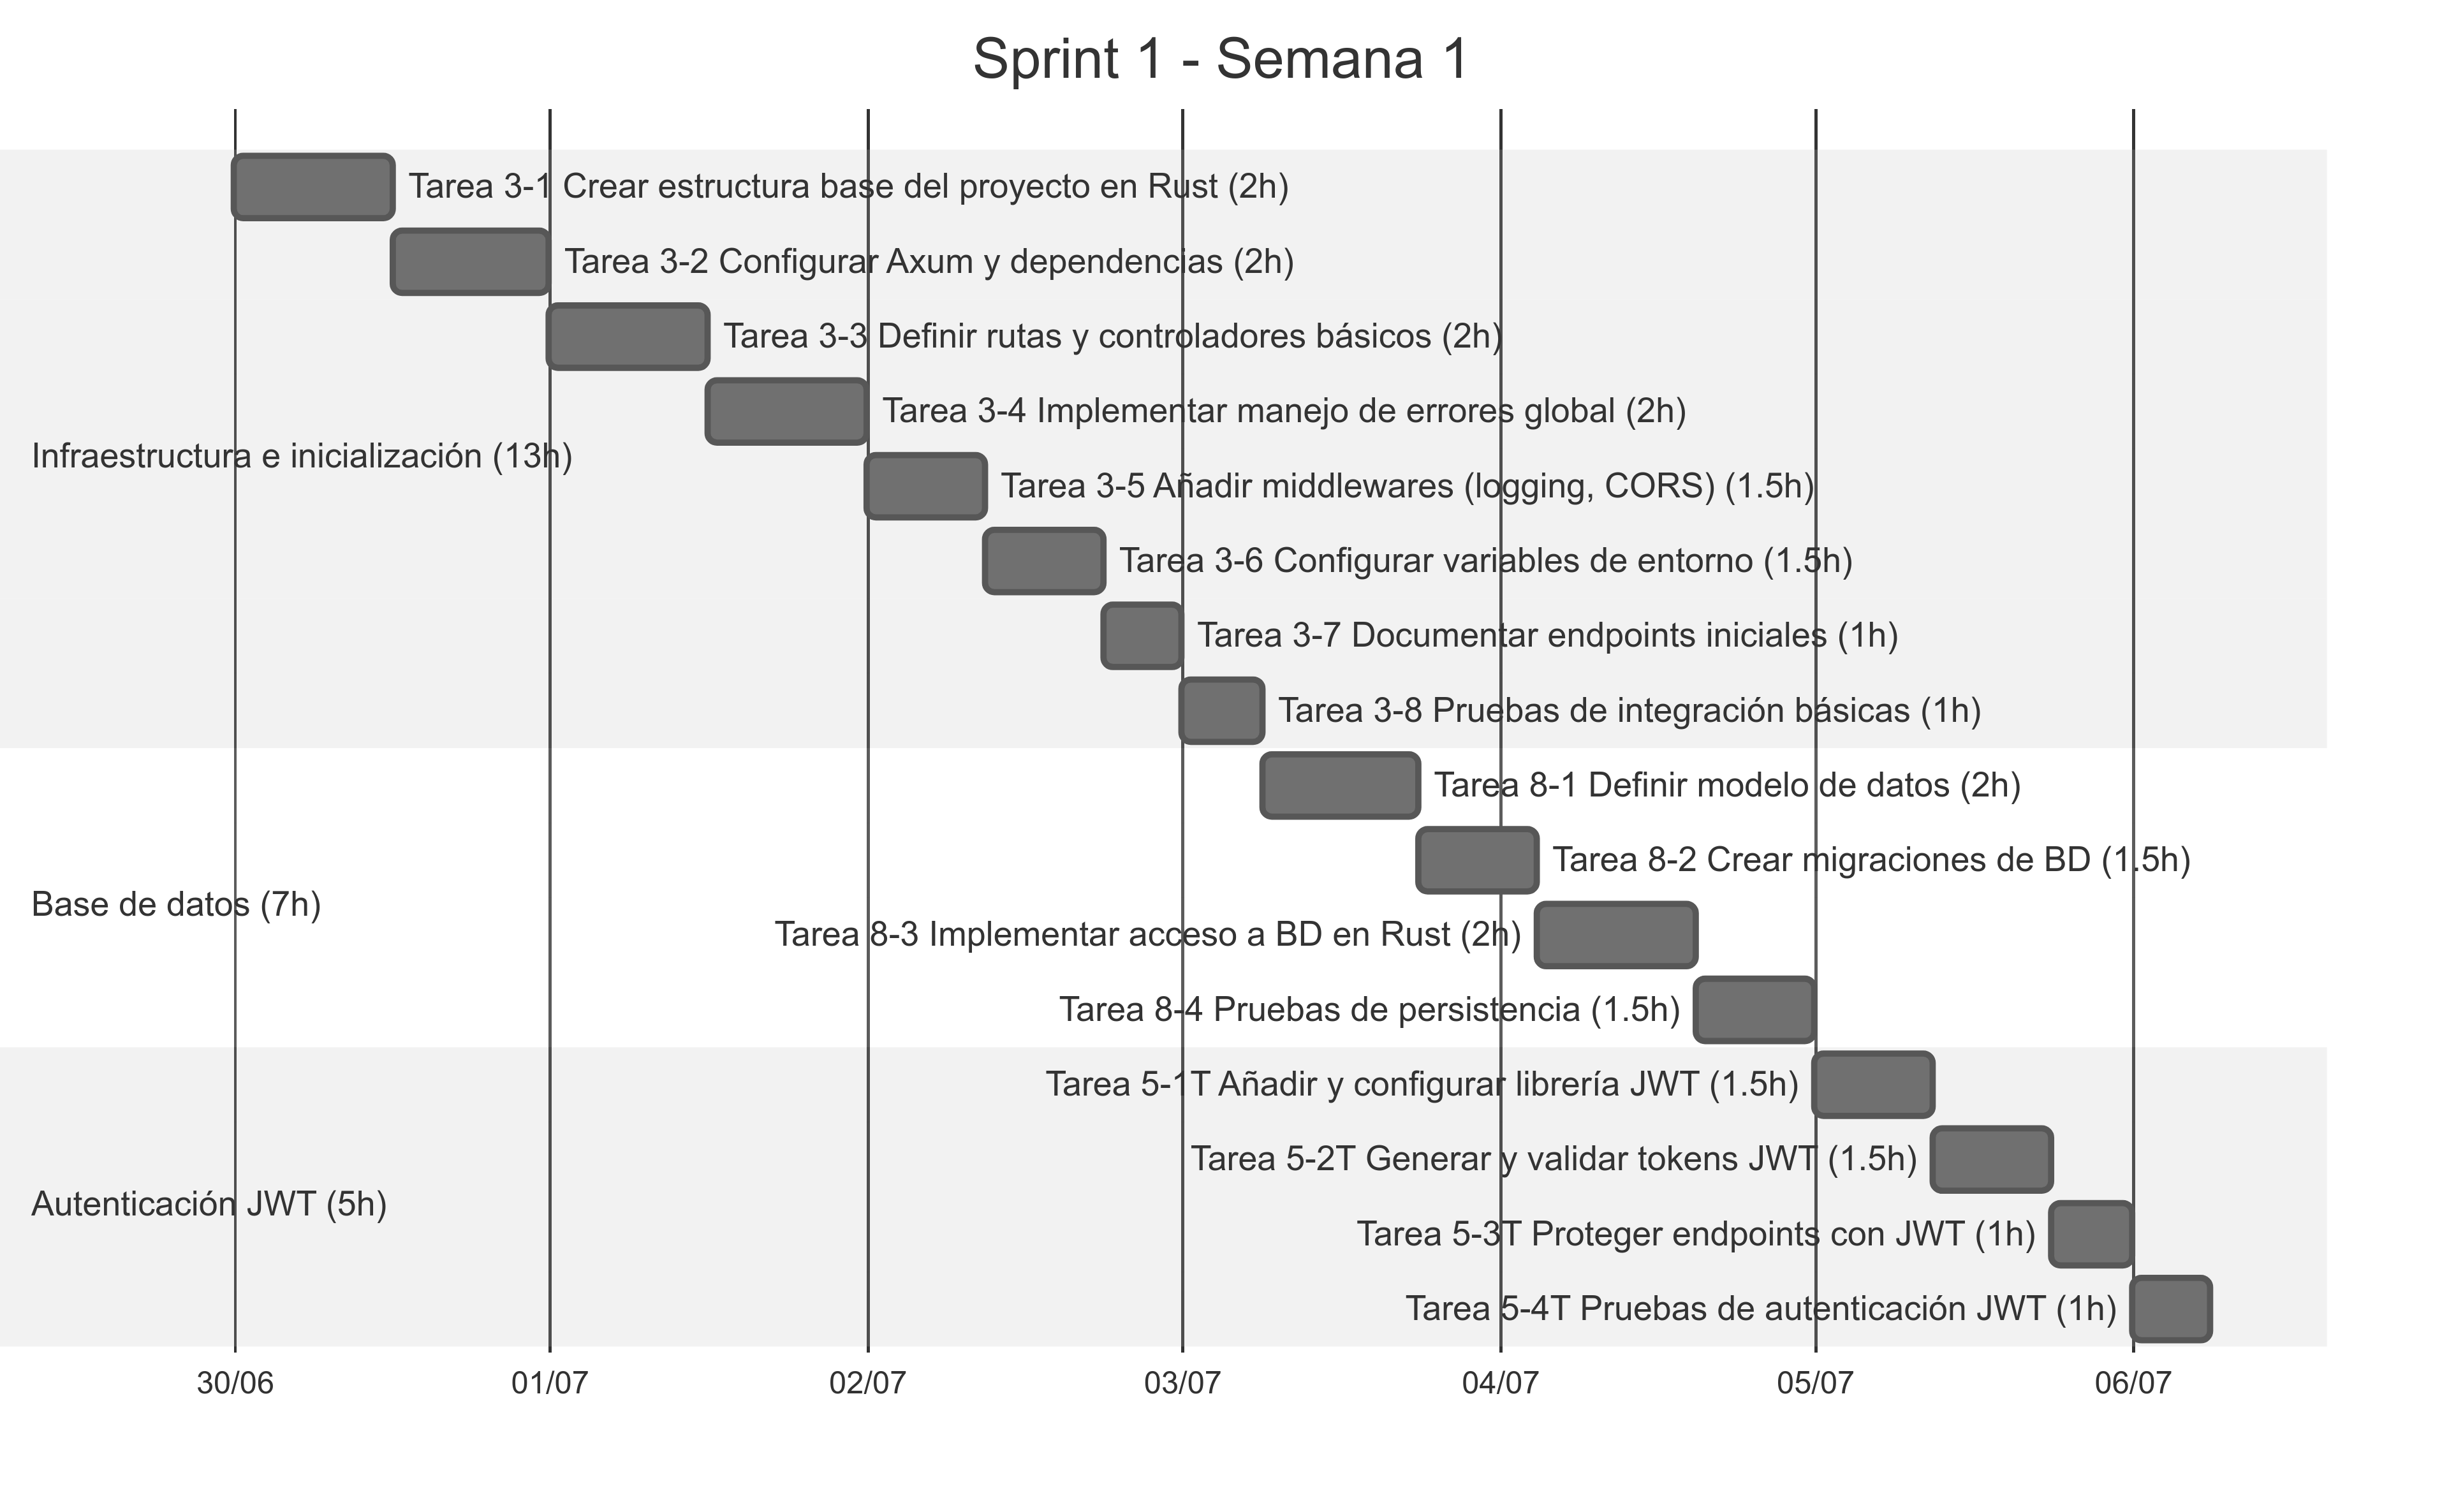
\includegraphics[width=0.8\textwidth]{assets/sprint1/sprint1-week1.png}
    \end{center}
    \caption{Diagrama de Gantt de las tareas de la primera semana del sprint}\label{fig:sprint1-week1}
\end{figure}

\begin{figure}[H]
    \begin{center}
        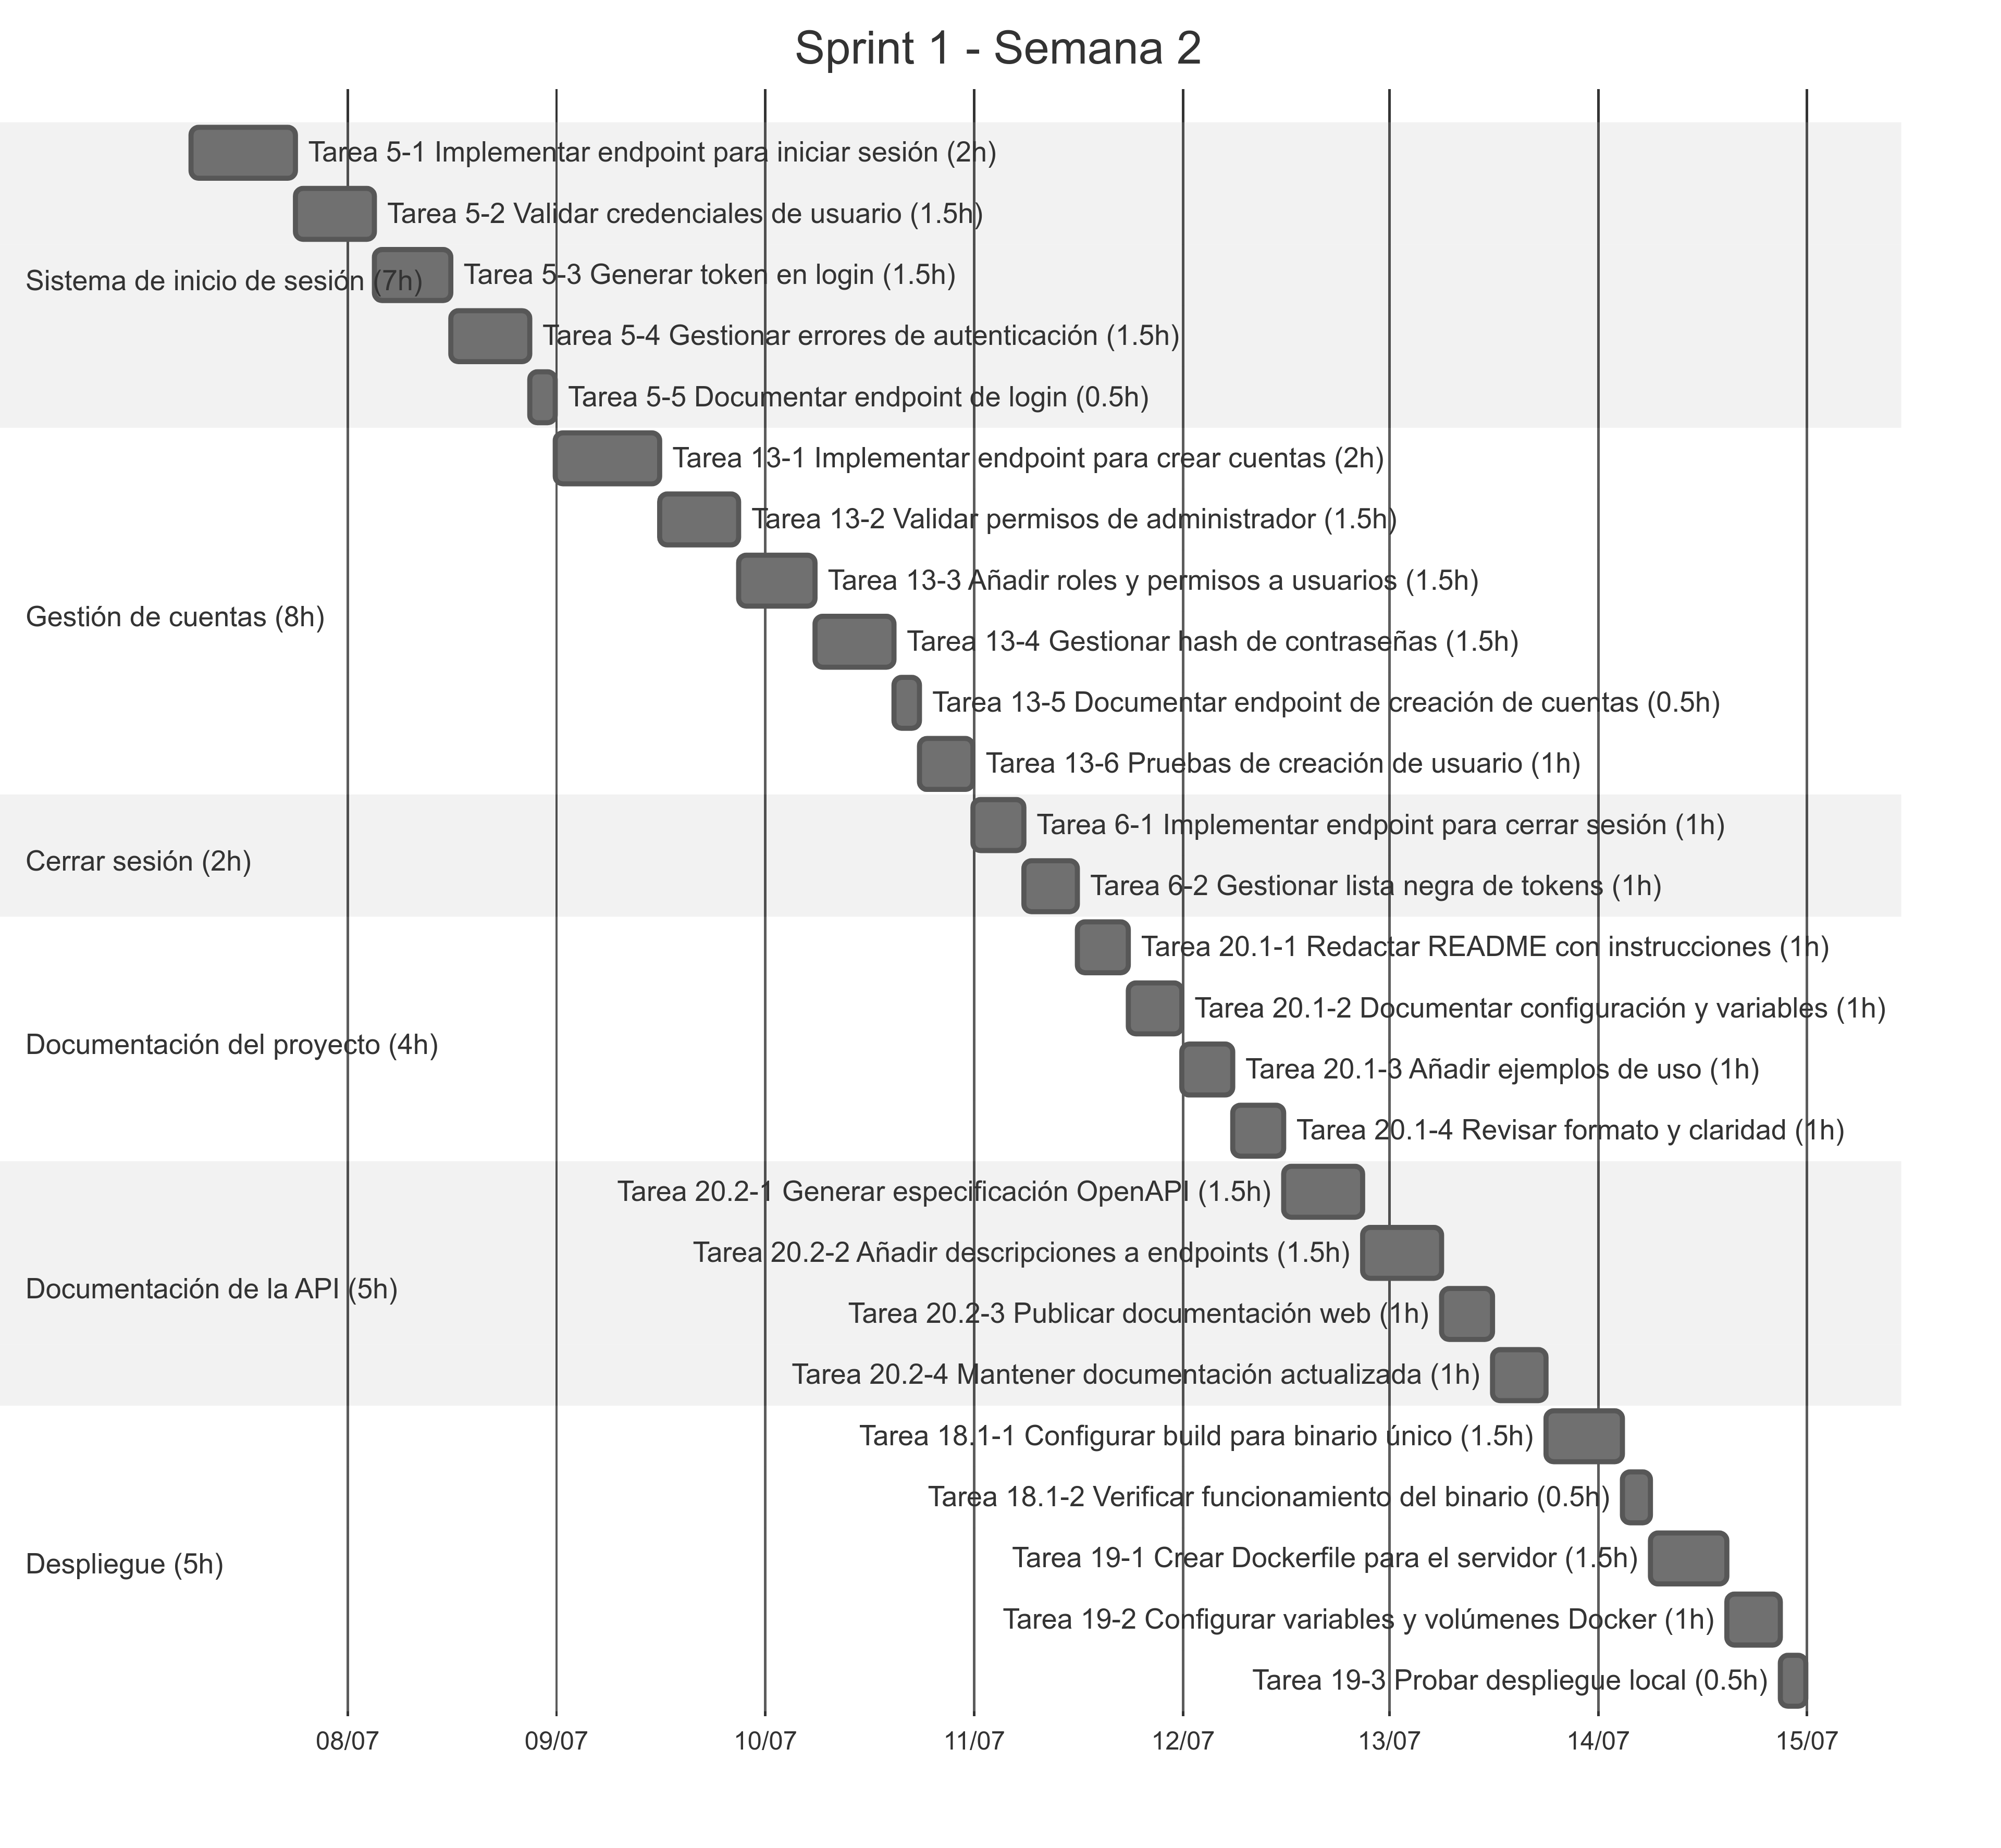
\includegraphics[width=0.8\textwidth]{assets/sprint1/sprint1-week2.png}
    \end{center}
    \caption{Diagrama de Gantt de las tareas de la segunda semana del sprint}\label{fig:sprint1-week2}
\end{figure}

Se ha seguido un orden lógico, en el que primero inicializaremos toda la capa de interfaz, en este caso nuestra API, junto con todas las dependencias que nos harán falta a la hora de documentar, errores no genéricos, variables de entorno, pruebas...

Después, se implementará el diseño de la base de datos. Una vez tenemos esta base, se implementarán las primeras funcionalidades, que van a ser la del inicio de sesión seguro, seguido de la gestión de cuentas. Para finalizar el sprint, se documentará todo al completo.

Para finalizar, configuraremos todo lo necesario para poder desplegar el servidor.
